\section{Введение}

\subsection{Аннотация}
    В качестве объекта исследования в рамках курсовой работы мной был выбран кейс, предложенный известным порталом по обмену знаниями Quora. На протяжении всего своего существования Quora сталкивается с нежелательным контентом, который ухудшает пользовательский опыт и усложняет работу всего сайта. Моя задача состоит в том, чтобы разработать универсальную расширяемую многофункциональную систему для распознавания и отсеивания такого токсичного контента.\\
    
    As an object of study in the course work I have chosen the case proposed by the well-known portal for the exchange of knowledge Quora. Throughout its existence, Quora encounters unwanted content that degrades the user experience and complicates the operation of the entire site. My task is to develop a universal expandable multifunctional system for the recognition and screening of such toxic content.
\subsection{Актуальность}

    Трудно переоценить своевременность и актуальность поднимаемой проблемы: каждый из нас каждый день сталкивается с неподобающим поведением со стороны других пользователей интернета. В основном, это вызвано анонимностью оставленных комментариев, однако мы не пойдем по пути деанонимизации, а будем бороться с проблемой путем автоматического определения и удаления спорного содержания. Полученное решение без проблем можно обобщить на другие области, например комментарии в соцсетях, отзывы на товары и т.п.

\subsection{Структура работы}

    	Моя работа будет разбита на две смысловые части. В первой мы подберем математическую модель, которая бы лучше всего подходила для поставленной задачи и достигала требуемого качества. Мы рассмотрим несколько вариантов решения и выберем лучший из них.
    	
    	Во второй части мы сконцентрируемся на реализации выбранной модели. Рассмотрим общие архитектурные решения для задач по машинному обучению и обработке данных, обозначим проблемные моменты, которые помешают масштабированию проекта, и в конечном итоге придем к наиболее удобной структуре проекта, которая бы поддерживала работу с несколькими математическими моделями, преобразователями данных, инструментами для статистического анализа и т.п.
\pagebreak
\subsection{Обозначения}
На протяжении всей работы я буду сопровождать текстовые выкладки иллюстрациями в виде блок-схем. В целом, обозначения в них довольно очевидны, однако, чтобы исключить неправильное понимание, уточним их.
Они будут состоять из следющих объектов:

\begin{table}[ht]
\caption{Обозначения в блок-схемах}
\centering
\begin{tabular}{*{2}{m{0.48\textwidth}}}
\hline
\begin{center}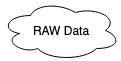
\includegraphics[height=40pt]{images/raw_digram_example}\end{center}&Необработанные данные, поступающие на вход программы. В случае с решением задачи от Quora ими являются формулировки вопросов, которые нужно профильтровать.\\\\
\begin{center}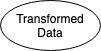
\includegraphics[height=36pt]{images/transformed_data_example}\end{center}&Данные, полученные нами из исходных некоторым преобразованием. Например, это может быть лемматизированный текст или вектор, характеризующий относительное семантическое положение слова.\\\\
\begin{center}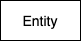
\includegraphics[height=30pt]{images/entity_example}\end{center}&Абстрактная сущность, которая в нашей архитектуре будет выполнять поставленную ей роль.\\
\end{tabular}
\label{tab:gt}
\end{table}

Как можно видеть, схемы довольно простые, и, в тоже время, функциональные.
\pagebreak
